\documentclass[11pt]{article}
\addtolength{\oddsidemargin}{-1.cm}
\addtolength{\textwidth}{2cm}
\addtolength{\topmargin}{-2cm}
\addtolength{\textheight}{3.5cm}

\usepackage[pdftex]{graphicx}
\usepackage{hyperref}
\usepackage{float}
\usepackage{cite}
\hypersetup{
	colorlinks=true,
	linkcolor=black,
	filecolor=magenta,
	urlcolor=cyan,
}

% define the title
\author{Team CodeX}
\title{Architecture Requirements Specification}

\begin{document}
	\setlength{\parskip}{6pt}
	
	% generates the title
	\begin{titlepage}
	
	\begin{center}
		% Upper part of the page       
		
\includegraphics[width=0.7\linewidth]{../Images/eVoting_Logo.png}\\[2cm]    
		\textsc{\LARGE Electronic Voting}\\[0.5cm]
		% Title
		\rule{\linewidth}{0.5mm} \\[1cm]
		{ \huge \bfseries User Manual}\\[0.5cm]
		\rule{\linewidth}{0.5mm} \\[1cm]
		
		% Author and supervisor
<<<<<<< HEAD
		
\includegraphics[width=0.5\linewidth]{../Images/TeamCodexLogo.jpg}\\[0.5cm]    	
=======
		
		
\includegraphics[width=0.5\textwidth]{../Images/TeamCodexLogo.jpg}\\[0.5cm]    	
>>>>>>> 9b25dd959830e00c0e449a84c7623c3e326c347b
		
		
		\begin{minipage}{0.4\textwidth}
			\begin{flushleft} \large
				Andreas {du Preez}
			\end{flushleft}
		\end{minipage}
		\begin{minipage}{0.4\textwidth}
			\begin{flushright} \large
				\emph{} \\
				12207871 
			\end{flushright}
		\end{minipage}
		
		
		\begin{minipage}{0.4\textwidth}
			\begin{flushleft} \large
				\emph{} \\
				Azhar {Mohungoo }
			\end{flushleft}
		\end{minipage}
		\begin{minipage}{0.4\textwidth}
			\begin{flushright} \large
				\emph{} \\
				12239799
			\end{flushright}
		\end{minipage}
		
		
		\begin{minipage}{0.4\textwidth}
			\begin{flushleft} \large
				\emph{} \\
				Gift {Sefako }
			\end{flushleft}
		\end{minipage}
		\begin{minipage}{0.4\textwidth}
			\begin{flushright} \large
				\emph{} \\
				12231097
			\end{flushright}
		\end{minipage}
		
		\textsc{\Large Stakeholders}\\[1cm]	
				
		\begin{minipage}{0.4\textwidth}
			\begin{flushleft} \large
				\emph{} \\
				Epi-Use Advance
			\end{flushleft}
		\end{minipage}
		\begin{minipage}{0.4\textwidth}
			\begin{flushright} \large
				\emph{} \\
				Roelof Nuade
			\end{flushright}
		\end{minipage}
		
	\end{center}
\end{titlepage}
	
	\renewcommand{\thesection}{\arabic{section}}
	\newpage
	
	\tableofcontents
	
	\textsc{}\\[1cm]
	
	\newpage

	\section{Architectural Requirements}
	\begin{figure}[H]
		\centering
		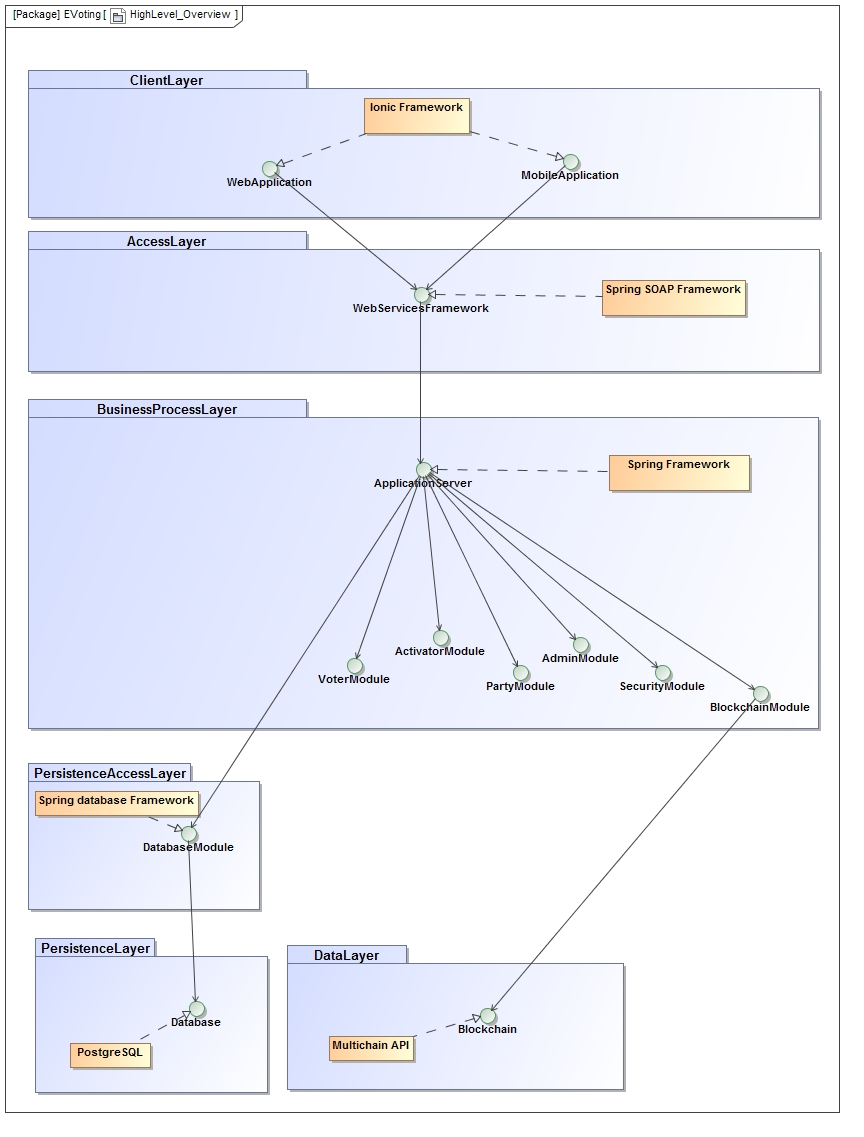
\includegraphics[width=0.75\linewidth]{../Images/System/HighLevel_Overview.jpg}
		\caption{High Level System Diagram}
	\end{figure}
	
	\newpage
	
	\subsection{Architectural Scope}
		\begin{enumerate}
		\item Supply a persistence framework which supports integration with databases and database technologies, and provides secure access to persistent data
		\item Support system flexibility in adding or removing existing modules without necessitating system shutdown
		\item Provide a reporting infrastructure, which is: distributed, consistent, accurate, timely, and reliable
		\item Supports system integration with front-end clients, the bare minimum of which should be a desktop web client and an Android mobile client
		\item Cater for concurrent stateless access to services to at least one hundred clients
		\item Provide functionality benchmarking infrastructure
		\item Provide integration with authentication frameworks
\end{enumerate}
	
	\subsection{Quality Requirements}
		\begin{enumerate}
	\item \textbf{Convenience:} The system shall allow the voters to cast their votes quickly, in one session, and should not require many special skills or intimidate the voter.
	
	\item \textbf{User-Interface:} The system shall provide an easy-to-use user-interface. Also, it shall not disadvantage any candidate while displaying the choices.
	
	\item \textbf{Transparency:} Voters should be able to possess a general knowledge and understanding of the voting process.
	
	\item \textbf{Accuracy:} The system shall record and count all the votes and shall do so correctly.
	
	\item \textbf{Eligibility:} Only authorized voters, who are activated, should be able to vote.
	
	\item \textbf{Uniqueness:} No voter should be able to vote more than once for the same poll.
	
	\item \textbf{Auditability:} It should be possible to verify that all votes have been correctly accounted for in the final election tally, and there should be reliable and demonstrably authentic election records, in terms of physical, permanent audit trail, which should not reveal the user’s identity in any manner.
	
	\item \textbf{Confirmation:} The voter shall be able to confirm clearly how his vote is being cast, and shall be given a chance to modify his vote before he commits it.
	
	\item \textbf{No Over-voting:} The voter shall be prevented from choosing more than one party.
	
	\item \textbf{Documentation and Assurance:} The design, implementation, and testing procedures must be well documented so that the voter-confidence in the election process is ensured.
	
	\item \textbf{Cost-effectiveness:} Election systems should be affordable and efficient.
	
	\item \textbf{Authenticity:} Ensure that the voter must identify himself (with respect to the registration database) to be entitled to vote.
	
	\item \textbf{Anonymity:} Ensure that votes must not be associated with voter identity.
	
	\item \textbf{System Integrity:} Ensure that the system cannot be re-configured during operation.
	
	\item \textbf{Data Integrity:} Ensure that each vote is recorded as intended and cannot be tampered with in any manner, once recorded. Votes should not be modified, forged or deleted without detection.
	
	\item \textbf{Privacy:} No one should be able to determine how any individual voted.
	
	\item \textbf{Reliability:} Election systems should work robustly, without loss of any votes, even in the face of numerous failures, including failures of voting machines and total loss of network communication. The system shall be developed in a manner that ensures there is no malicious code or bugs.
	
	\item \textbf{Availability:} Ensure that system is protected against accidental and malicious denial of service attacks.
	
	\item \textbf{Simplicity:} The system shall be designed to be extremely simple, as complexity is the enemy of security.
	
	\item \textbf{System Accountability:} Ensure that system operations are logged and audited.
	
	\item \textbf{Authentication and Control:} Ensure that those operating and administering the system are authenticated and have strictly controlled functional access on the system.
	
	\item \textbf{Distribution of Authority:} The administrative authority shall not rest with a single entity. The authority shall be distributed among multiple administrators, who are known not to collude among themselves.
\end{enumerate}

	
	\subsection{Integration and Access Channel Requirements}
		\begin{itemize}
		\item The aim of the Electronic Voting system is to allow users to participate in elections remotely, i.e. that they do not have to go into a voting station to cast their vote. The easiest way to achieve this is by providing both a web interface as well as an Android interface (seeing as Android is currently the most widely used operating system for mobiles in South Africa). 
		
		\item The ultimate goal is that users will be able to easily download and use the Android application from the Google Play Store. The web interface will obviously be accessed from the users preferred browser – so we will, whilst developing the system test it currently with multiple web browsers too to ensure that users are never disadvantaged according to their preferred browser.  
		
		\item The Electronic Voting system requires the use of Blockchain to maintain elections, votes, voters and candidates – as well a generic version of the system which allows participants to partake in surveys. 
		
		Blockchain Explained: 
		\begin{enumerate}
			\item[] The Blockchain is a shared transparent ledger on which the entire Bitcoin network relies. All confirmed transactions are included in the block chain. 
			
			Once a transaction is entered in the Blockchain, it can never be erased or modified. Blockchain also allows us to ensure that voters cannot vote more times than allowed. So once a vote has been cast, a voter is sure that their vote was counted for the right candidate. 
		\end{enumerate}
		
		\item The backbone of our Blockchain servers will be the Linux based MultiChain implementation which will allow us to create and manage nodes of the which we will use to implement our own local Blockchain. 
		
		\item The backend of the system will be implemented using Java since it integrates easily with the Spring Framework.   			
		
		\item PostgreSQL will be used for the database as it provides several external authentication tools and it provides support for the use of JSON(this is also how MultiChain communicates with browsers in the MultiChain Explorer that provides a visual representation of the local blockchain), which will assist with the integration of the server-side communication. 
		
		\item RESTful
		\begin{enumerate}
			\item The front end will communicate with the backend using a RESTful webservice. REST (REpresentational State Transfer) is an architectural style, and an approach to communications that is often used in the development of Web services. 
			
			\item REST uses a smaller message format than SOAP, which uses XML for all messages, which makes the message size much larger, and thus less efficient. This means REST provides better performance, as well as lowers costs over time. Moreover, there is no intensive processing required, thus it’s much faster than traditional SOAP.
		\end{enumerate}
\end{itemize}
	
	\newpage
	
	\subsection{Architectural Constraints}
		\begin{enumerate}
	\item Blockchain
	\begin{enumerate}
		\item We're using Multichain to represent the Blockchain component of the Electronic Voting system. The Multchain allows us to manage transactions that happen when a user casts a vote, instantiation and management of all the types of nodes in the chain as well retrieving the balances of all the Party nodes when required. 
		
		\item The constraint which has been imposed with regards to the Multichain servers is the fact that there is only Linux support for the servers. 
		
	\end{enumerate}
	
	\item Ionic
	\begin{enumerate}
		\item The Ionic framework allows for develop hybrid mobile applications. The biggest drawback with Ionic since it is not native (Android or iOS) development is that it must support multiple platforms with a single codebase. In the greater scheme of things this is a minor issue since most web browsers are webkit based.
		
		\item Hybrid development is best when there won’t be intense functionality such as 3D graphics on the application/website itself. So the architectural constraint with regards to the front end is basically that interfaces of the system should be basically be used for simple message passing.  
	\end{enumerate}
	
	\item Postgre
	\begin{enumerate}
		\item Postgre databases have an inherent speed constraint because of its representation of database records as fully instantiated objects in code, this might slow down pre-processing of the system, more especially when it is compared to MySQL. 
		
		\item Does not support the entire ANSI SQL 92' standard, much less the ANSI SQL 99' standard
	\end{enumerate}
	
	\item Android 
	\begin{enumerate}
		\item The front end of the system will be a website component as well as an android component. The Android component will only be supported by Android 4.3 to more recent releases. 
	\end{enumerate}
\end{enumerate}

	
	\newpage
	
	\subsection{Architectural Patterns and Styles}
		The project implementaton will use MVC (Model View controller) pattern for the project. As the following benefits will be utilised provided by implementing MVC
	\begin{enumerate}
		\item Separation of concerns thus allowing:
		\begin{enumerate}
			\item Re-use of the business logic across the platform 
			\item Multiple user interfaces can be developed without concerning the codebase
		\end{enumerate}
		
		\item Developer specialisation and focus:
		\begin{enumerate}
			\item The developers of UI can focus exclusively on the UI screens without bogged down with business logic.
			\item The developer of Model / business can focus exclusively on the business logic implementations, modifications, updations without concerning the look and feel and it has nothing to with business logic.
		\end{enumerate}
		
		\item Parallel development by separate teams:
		\begin{enumerate}
			\item Business logic developers can build the classes, while the UI developers can involve in designing UI screens simultaneously, resulting the interdependency issues and time conservation.
			\item UI updations can be made without slowing down the business logic process.
			\item Business logic rules changes are very less that needs the revision / updations of the UI.
		\end{enumerate}
		
		\item Multiple view support:
		\begin{enumerate}
			\item Due to the separation of the model from the view, the user interface can display multiple views of the same data at the same time.
		\end{enumerate}
		
		\item Change Accommodation:
		\begin{enumerate}
			\item User interfaces tend to change more frequently than business rules. (different colors, fonts, screen layouts, and levels of support for new 									devices such as cell phones or PDAs) Because the model does not depend on the views, adding new types of views to the system generally does not affect the model. As a result, the scope of change is confined to the view.
		\end{enumerate}
	\end{enumerate}
	
	\subsection{Architectural Tactics and Strategies}
		\begin{enumerate}
		\item\textbf{Authentication}\newline
		All of our web service methods requires that the requesting object contains an ID number and a password. We will be authenticating the user to see if he/she is in fact registered, and if he/she has access to our methods' functionality and will be denied otherwise.
		
		\item\textbf{Encryption}\newline
		To ensure a safe and secure system, we will be encrypting the users' password on the client side before sending it to the server side. We won't be decrypting the password, nor will we know how to decrypt it. The encrypted passwords will directly be stored in our database as a string. As soon as a user is to be authenticated, the encrypted password strings will be matched to see if the password is the same.\newline Encryption will also be used to encrypt the voting node's address and party node's address. This we will be decrypted on the server side.
		
		\item\textbf{Database Indexing}\newline
		All of our database tables will have primary keys, and also foreign keys linking to other tables.
		
		\item\textbf{Database Integrity}\newline
		To ensure database data fault prevention, each database base will have its respective audit table. Inside each audit table, there will be columns for: the type of modification (insert/update/delete); a date column when the modification was made; a column specifying who did the modification (Admin, Node1, Node2 etc); and the rest of the columns will all of the original table's columns. Its important to note that no one, not even the Administrator, will be able to delete rows from the audit table.
\end{enumerate}	
	
	\newpage
	
	\subsection{Reference Architectures and Frameworks}
		\begin{enumerate}

		\item \textbf{Spring Boot} is one of the features of Spring Framework version 4.0 which gives us a way to improve Java applications quickly and simply through an embedded server – this means we can expose components such as REST services independently. This framework will prove useful when deploying the Electronic Voting system. 
		
		\item \textbf{AngularJS} is a Javascript framework that be added to a HTML web page. AngularJS extends HTML attributes and binds data to HTML. It will be used to build highly interactive web pages for the Electronic Voting system. 
		
		\item \textbf{Bootsrap} is a HTML, CSS, and Javascript framework for developing responsive mobile-first web sites. We will use when writing the front-end of the web site and Android interface of the Electronic Voting system. 
		
		
\end{enumerate} 
	
	\subsection{Technologies}
		The technologies that will be implemented in the system to achieve the desired outcome and allow not only successful completion of the project but doing it in the most effective and efficient manner. The technologies are stated with an explaination why they were chosen for this project.
	\begin{enumerate}
		\item \textbf{AngularJS:} 
		\begin{enumerate}
			\item Implements MVC (Model View Controller) which the is Architectural Pattern that is to be implenmented. Angular manages the components and serves as a pipeline to connect them.
			\item Uses HTML to define the interface which is more intuitive and less convoluted than defining the interface in JavaScript. It is also less brittle to reorganize than an interface written in JavaScript.
			\item The data models are POJO (plain old JavaScript objects) which means there is no need for extraneous getter and setter functions.
			\item Behaviour with directives will allow us to invent our own HTML elements by putting all the DOM manipulation code into directives. They are separated out of the MVC application, therefore the MVC application only concerns itself with updating the view with the new data.
			\item Flexibility with filters which will allow the filters to be standalone functions that will be separate from the applicaiton similar to directives, but are only concerned with data transformations such as formatting numbers or reversing the order of an array.
			\item Consise code because of all the aforementioned points will cause less code to be written. No need to write a MVC pipeline. The view is defined just by HTML, models are simpler because there are no extra getter and setter functions. Data binding means there is no need to put data into the data manually. Parrellel team work is possible since the directives are separate from the application code. The filters allow data manipulation on the view level without changing the controllers.
			\item AngularJS can be unit tested by mocking data into the controller and measuring the output and behaviour.
		\end{enumerate}
		
		\item \textbf{PostgreSQL:}
		\begin{enumerate}
			\item Immunity to over-deployment 
			\item Better support than the proprietary vendors 
			\item Stability and reliability
			\item Extensible 
			\item Cross platform
			\item Designed for high volume environments
			\item GUI database design and administration tools
		\end{enumerate} 
		
		\item \textbf{Maven:}
		\begin{enumerate}
			\item Making the build process easy 
			\item Providing a uniform build system
			\item Providing quality project information
			\item Providing guidelines for best practices development
			\item Allowing transparent migration to new features
		\end{enumerate}
		
		\item \textbf{HTML:}
		\begin{enumerate}
			\item Supported by both platforms to be implemented web interface and andriod
		\end{enumerate}
		
		\item \textbf{Bootstrap:}
		\begin{enumerate}
			\item Easy to use
			\item Will implement the CSS to allow adjustment to all platforms
			\item Speed of development
			\item Responsiveness 
			\item Consistency
			\item Customizable
			\item Support
		\end{enumerate}
		
		\item \textbf{Java:}
		\begin{enumerate}
			\item Simple to use with built in functions to assist and make it more simple to use
			\item Object-Oriented to assist the MVC (Model View Controller) architecture
			\item Multi-threaded to assist with the scale of the project
			\item Distrubed which will be needed for the implementation of BlockChain
			\item Portable as it is platform independent
		\end{enumerate}
		
		\item \textbf{JHipster:}
		\begin{enumerate}
			\item Facilitate the front end of the project
		\end{enumerate}
		
		\item \textbf{MultiChain:}	
		\begin{enumerate}
			\item This what will be used to implement the BlockChain
		\end{enumerate}
	\end{enumerate}
	
\end{document}